\subsection{Profiling}
Profiling a system allows a user or system administrator to see which functions are being called the most frequently.  Oprofile \cite{levon} is a profiler that can profile both application and kernel functions, by registering with the Performance Monitoring Unit (PMU) on the CPU.  The PMU will track hardware counters and will notify the registered profiler when a specific hardware counter reaches a threshold set by the profiler \cite{mucci}.  When Oprofile receives notification, through an NMI, it will record the PC and other information about the system, and over time will have the most frequently called function when the specified hardware event occured.  Some typical hardware events counters are:  TLB miss, LLC Cache miss, or CPU instructions retired.   Other profilers like OSprof use latency distribution analysis [7].  As function calls are entered and exited to or from the stack, the profiler tracks the start and end time of the functions.

\indent The difficulties with running a profiler like Oprofile in a virtualized guest is that the hardware counters in the guest may not be available for all hypervisors \cite{buell1}.  Additionally, the guest is not guaranteed to receive interrupts in a correct order.   Tracking the wall-clock time and CPU time on virtual machines is extremely difficult and there are many additions in the hypervisor to help guest machines accurately track time.  Usually to profile a kernel a patch or configuration change is needed to enable profiling, which makes it difficult on production systems.

\indent In virtualization there are 2 types of profiling:  Guest-wide profilers only profile a single guest (or domain), and System-wide which monitors all guests and the VMM \cite{du1}.  In order to provide Guest-wide profiling for virtual systems, the profiler runs in the guest and the VMM needs to provide synchronous delivery of interrupts from the hardware to the guest machines.  For System-wide profiling the profiler runs in the VMM and requires interaction between the guest OS and VMM.  Specifically, the VMM needs to know which application and kernel functions are running on the guest machine at the time of the interrupt.

\indent Xenoprof uses Oprofile to provide the profiling and uses Xen's hypercalls to share information between the guest and Xen Hypervisor.  The Xenoprof toolkit supports system-wide coordinated profiling in a Xen environment.  The underlying Oprofile uses statistical profiling across domains and can track functions running in the user space, kernel space, and in the hypervisor.  Xenoprof provides a performance event interface which maps physical hardware events to virtual HW counters \cite{santos, menon2}.   The guest-level profiling registers with the virtual CPU, and the hypervisor registers with the physical hardware.  Since it is not possible to call the domain level virtual interrupt handler synchronously, Xenoprof collects the samples for the guest domain and logs them to that specific domain buffer, and then Xenoprof sends a virtual interrupt to the guest domain.

\indent In KVM, a Linux Kernel VM subsystem, a customized profiler can implement both guest-wide and system-wide profiling \cite{du2}.  Linux perf is another profiler that runs in the Host Linux on KVM, and can measure software and harware event counters as well as tracing.  It is aware of the memory layout of the guest and can monitor the Kernel space of the guest VM, but not its user-space application. 

\begin{comment}
\indent VMware ESX sever strives to provide a complete full virtualization including hardware counters to allow any guest profiling to work as if it were on native hardware.  VMware creates a virtual timer for the guest OS, but the profiler may need relative time difference and track only time on the Virtual CPU.  Additionally, there needs to be a way to efficiently and accurately emulate interrupt events from the virtual machine to the host. These techniques are classified as speculative and non-speculative events, and the Hypervisor may try to give the guest a complete view of system in order to run any Profiler in the unmodified guest OS.  VMware provides VMKperf in order to profile the hypervisor, but does not profile the guest OS.
\end{comment}

\indent Profiling results also require manual inspection and may not show how interference from other parts of the system or virtual machines impact the guest machine \cite{traeger, knapp1}.  Additionally the user running the profiler needs to have some "guess" or prior knowledge about what event to sample, and the desired freqency of the sample.  Should the user sample Cache miss, TLB miss, or some other counter?  As more events are profiled, the more perturbation is encounted.  In a virtual environment a user may need to start several profilers on several virtual machines each monitoring various hardware counters, system state, and applications.  Only after several runs in many different configurations and manual inspection could an advanced administrator make some determination as to the root cause of the problem. 

\subsection{Performance Monitoring}
Modern operating systems have a method of monitoring the performance of the system.  These statistics are tracked in the kernel to track access to resources, and are not (necessarily) related to the PMU on the CPU.  For example a specific CPU may track hard events such as L2 cache miss, or TLB cache miss, but the kernel will track time spent reading or writing to a physical disk, or virtual memory cache information.

\indent In a Linux OS there are administration tools such as top, iostat, ps, and vmstat.  
Windows uses \emph{Performance Monitor} or \emph{Resource Monitor} to show the current performance.  
Most kernels will write statistics when each resource is used, and these tools read and analyze the kernel data about resource usage, through the method provided by the kernel.
By examining these counters and aggregating the data with tools, an administrator can see the current threads and how each of the resources are being used. 

\indent When a system is virtualized, the guest OS kernel only tracks the statistics from its own viewpoint.  
In other words, the resource statistics are for the virtualized resource, and not the physical resource.

\indent When monitoring virtualized resources, the counters only measure the virtual resource.  
As our tests will show, they do not necessarily aggregate as expected.  
The counters do not collect information from external guests or show the interference from external guests or the hypervisor.  
In order to accurately analyze performance issues on complex virtualized systems, we need to collect and analyze resource usage from all systems and the hypervisor.  
We need the ability to perform System-wide performance monitoring similar to the System-wide profiling available.

\subsubsection{Linux Tools}
\indent On Linux these resource counters are tracked in the /proc filesystem, which is a dynamic view into the kernel data structures and statistics \cite{proc}.  
For example \emph{/proc/stat} contains statistics about the time (since boot) that the the CPU was idle, running in user mode, or running in kernel mode.
By running a test load and examining the /proc filesystem or using the tools, one can reasonably determine the resources used and which process or thread is using them.  
In many cases these tools can quickly narrow the scope of possible problems for a degraded system. 

\begin{figure}[h]
\begin{Verbatim}
top - 15:57:05 up 109 days, 23:54,  6 users,  load average: 0.12, 0.17, 0.11
Tasks: 164 total,   1 running, 163 sleeping,   0 stopped,   0 zombie
Cpu(s):  6.0%us,  0.7%sy,  0.0%ni, 93.3%id,  0.0%wa,  0.0%hi,  0.0%si,  0.0%st
Mem:   2062348k total,  1868648k used,   193700k free,   185776k buffers
Swap:  2095100k total,   389996k used,  1705104k free,   699236k cached

  PID USER      PR  NI  VIRT  RES  SHR S %CPU %MEM    TIME+  COMMAND            
  999 root      20   0 94876  52m 4900 S  4.0  2.6 373:01.16 Xorg               
 5362 deron     20   0  317m  92m  62m S  2.0  4.6 300:20.40 soffice.bin        
25333 deron     20   0  140m  15m 5684 S  1.0  0.8   3:33.53 gnome-terminal     
 1859 deron     20   0  166m 5820 4028 S  0.3  0.3   3:15.13 metacity           
\end{Verbatim}
\caption{\emph{top} collects information from Linux kernel through \emph{proc} and displays infromation about CPU, Memory, and processes}
\label{fig:top}
\end{figure}

\subsubsection{Windows Peformance Tools}
On Windows OS the counters are similar where the counters are tracked by the Windows kernel about processes and threads.  Then a userspace API \cite{winperf} is presented and a graph or report GUI administration tool can display any number of statistics about the system.  Similar to the /proc file system in Linux and administration tools there is little or no information provided about the overhead and interference from external layers.

\begin{figure}[!h]
  \begin{center}
  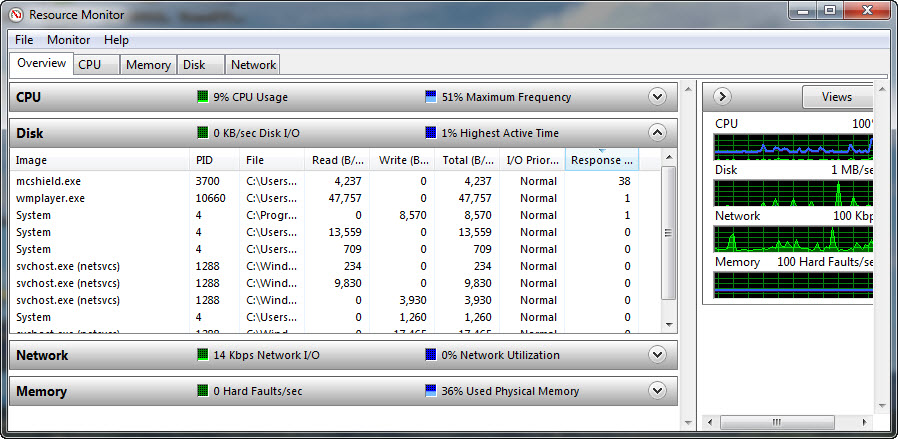
\includegraphics[width=6in]{images/ResourceMonitor.jpg}
  \caption{Microsoft Windows Resource Monitor.  Reads data from winperf API tracked in Windows kernel}
  \label{resourceMonitor}
  \end{center}
\end{figure}

\subsubsection{Hypervisor Peformance Tools}
Similar tools have been created in the hypervisor, \emph{xentop} for Xen and \emph{esxtop} for VMware, to show each virtual machine running and the resources that the entire machine is using.  
These tools use the same information from the \emph{proc} filesystem as VMware and Xen use a Linux based kernel.  
From this view we can see the guest machines, and the hypervisor, but we can't easily determine how they impact each other.  There is also no way to relate a virtual process running in the guest machine from the hypervisor tools.  The hypervisor has no access to the guest information.
Even if the these could show everything running in the guest machines, the administrator for the hypervisor and guest machines are different people or even completely different organizations. 

\begin{figure}[h]
\begin{Verbatim}

xentop - 17:07:00   Xen 4.2.2-23.el6
5 domains: 3 running, 2 blocked, 0 paused, 0 crashed, 0 dying, 0 shutdown
Mem: 4182752k total, 4182236k used, 516k free    CPUs: 4 @ 2133MHz
      NAME  STATE   CPU(sec) CPU(%)     MEM(k) MEM(%)  MAXMEM(k) MAXMEM(%) 
  Domain-0 -----r      78969   16.9    2035712   48.7    2097152      50.1    
  Test_VM1 -----r	    6474   11.5     524288   12.5     524288      12.5     
  Test_VM2 -----r	    4642   12.7     524288   12.5     524288      12.5 
  Test_VM3 --b---	    4210    0.1     524288   12.5     524288      12.5     
  Test_VM4 --b---	    4137    0.1     524288   12.5     524288      12.5  
\end{Verbatim}
\caption{\emph{xentop} 4 Guest domains. 2 are actively running and 2 are blocked.}
\label{fig:xentop}
\end{figure}

\subsubsection{Steal Time - Complete View}
Due to the fact that the hypervisor has one view of the system, and the virtualized guests have a different view of the system, the Xen Hypervisor has added a \emph{steal time} statistic and made it available to the guest operating systems.New linux distributions have implemented this new kernel option as \emph{steal: involuntary wait} \cite{proc}.  Additionally administrative tools top, sar, and vmstat have all implemented this new counter.  
On most systems top will show as '0.0\%st' (Figure ~\ref{fig:top}), but if it is running on a Xen Hypervisor the paravirtualized guest will communicate with the hypervisor and collect information. Amazon cloud uses Xen and this has become a valuable tool for guest to determine if they are having performance problems from external interference \cite{netflix}.

\subsection{Definitions}
\begin{description}
  \item[Hypervisor] A thin kernel layer that abstracts the hardware from the virtual guests.\\
  \item[VMM] Virtual Machine Manager. A kernel and OS that manages access to the hypervisor.  In Xen this is Dom0.\\
  \item[Guest] A complete OS (with applications) that is running under a hypervisor.  In Xen this is DomU.\\
  \item[Vitual Resource]  A physical resource (such as Disk, CPU or memory) that is managed by a hypervisor and allocated to a guest.\\
  \item[Virtualized] Changing a physical system to a virtual guest system.\\
  \item[Overcommit] Assigning more resources than are phyiscally available.\\
  \item[System-wide profiling] Both the guest and VMM are profiled.\\
  \item[System noise] Interrupts from deamons or other kernel processes that need to perform some task. \cite{tsafrir}\\
  \item[Paravirtualization] A virtualization technique where the native instruction set is not completely implemented.  Usually the Guest OS needs to be modified to know it is virtualized. This is the technique used by Xen. \cite{vmwareMem, du1}
  \item[Working set] The size of most of the data an application needs.  For database servers if the working set can fit into RAM, it is much faster than going to disk and swapping data. 
  \item[Overhead] The additional cost (time) required for virtualization.  For each operation, there may be additional resources required to virtualize the operation instead of interacting directly with the hardware.
  \item[Snapshot] A complete state of the entire virtual machine saved to non-volatile disk for later use.  A snapshot is used to create a template or roll back to a previous state.
\end{description}
